\documentclass[12pt]{article}
\usepackage{graphicx}
\usepackage{placeins}


% acronyms for text or math mode
\newcommand {\ccast} {\mbox{\small CCAST}}
\newcommand {\cris} {\mbox{\small CrIS}}

\newcommand {\airs} {\mbox{\small AIRS}}
\newcommand {\iasi} {\mbox{\small IASI}}
\newcommand {\idps} {\mbox{\small IDPS}}
\newcommand {\nasa} {\mbox{\small NASA}}
\newcommand {\noaa} {\mbox{\small NOAA}}
\newcommand {\nstar} {\mbox{\small STAR}}
\newcommand {\umbc} {\mbox{\small UMBC}}
\newcommand {\uw}   {\mbox{\small UW}}

\newcommand {\fft}  {\mbox{\small FFT}}
\newcommand {\ifft} {\mbox{\small IFFT}}
\newcommand {\fir}  {\mbox{\small FIR}}
\newcommand {\fov}  {\mbox{\small FOV}}
\newcommand {\for}  {\mbox{\small FOR}}
\newcommand {\ict}  {\mbox{\small ICT}}
\newcommand {\ils}  {\mbox{\small ILS}}
\newcommand {\igm}  {\mbox{\small IGM}}
\newcommand {\opd}  {\mbox{\small OPD}}
\newcommand {\rms}  {\mbox{\small RMS}}
\newcommand {\zpd}  {\mbox{\small ZPD}}
\newcommand {\ppm}  {\mbox{\small PPM}}
\newcommand {\srf}  {\mbox{\small SRF}}
\newcommand {\sdr}  {\mbox{\small SDR}}

\newcommand {\ES} {\mbox{\small ES}}
\newcommand {\SP} {\mbox{\small SP}}
\newcommand {\IT} {\mbox{\small IT}}
\newcommand {\SA} {\mbox{\small SA}}

\newcommand {\ET} {\mbox{\small ET}}
\newcommand {\FT} {\mbox{\small FT}}

% abbreviations, mainly for math mode
\newcommand {\real} {\mbox{real}}
\newcommand {\imag} {\mbox{imag}}
\newcommand {\atan} {\mbox{atan}}
\newcommand {\obs}  {\mbox{obs}}
\newcommand {\calc} {\mbox{calc}}
\newcommand {\sinc} {\mbox{sinc}}
\newcommand {\psinc} {\mbox{psinc}}
\newcommand {\std} {\mbox{std}}

% symbols, for math mode only
\newcommand {\wn} {\mbox{cm$^{-1}$}}
\newcommand {\lmax} {L_{\mbox{\tiny max}}}
\newcommand {\vmax} {V_{\mbox{\tiny max}}}

\newcommand {\tauobs} {\tau_{\mbox{\tiny obs}}}
\newcommand {\taucal} {\tau_{\mbox{\tiny calc}}}
\newcommand {\Vdc}  {V_{\mbox{\tiny DC}}}

\newcommand {\rIT} {r_{\mbox{\tiny\textsc{ict}}}}
\newcommand {\rES} {r_{\mbox{\tiny\textsc{es}}}}
\newcommand {\robs} {r_{\mbox{\tiny obs}}}

\newcommand {\rITobs} {r_{\mbox{\tiny\textsc{ict}}}^{\mbox{\tiny obs}}}
\newcommand {\rITcal} {r_{\mbox{\tiny\textsc{ict}}}^{\mbox{\tiny cal}}}

\newcommand {\ITmean} {\langle\mbox{\small IT}\rangle}
\newcommand {\SPmean} {\langle\mbox{\small SP}\rangle}


\title{DRAFT VERSION \\
  \vspace{5mm}
  Deconvolution and Translation \\
  Between High Spectral Resolution  \\
  IR Sounders \\
}

\author{Howard E.~Motteler \\
  \\
  UMBC Atmospheric Spectroscopy Lab \\
  Joint Center for Earth Systems Technology \\
}

\date{\today}
\begin{document}

\maketitle

\section{Introduction}

Upwelling infrared radiation as measured by the {\airs}, {\iasi},
and {\cris} sounders is a significant part of the long term climate
record.  We would like to treat this information as a single data
set but the instruments have different spectral resolutions, channel
response functions, and band spans.  To address this problem we
consider several channel radiance translations: {\iasi} to CrIS,
{\iasi} to {\airs}, {\cris} to {\airs}, and {\airs} to {\cris}.

Translation from {\airs} to {\cris} presents a special challenge
because while {\cris} and {\iasi} are Michaelson interferometers
with single response functions, {\airs} is a grating spectrometer
with a distinct response function for each channel.  We take
advantage of detailed knowledge of the {\airs} spectral response
functions (SRFs) to deconvolve {\airs} channel radiances to a
resolution enhanced intermediate representation.

The translations are validated by comparisons with calculated
reference truth.  For example to test the {\iasi} to {\airs}
translation, we start with 49 fitting profiles spanning a
significant range of atmospheric conditions.  Upwelling radiance is
calculated at a 0.0025 {\wn} grid with kcarta over a band spanning
the {\airs} and {\iasi} response functions.  ``True {\airs}'' is
calculated from this by convolving the kcarta radiances with
tabulated {\airs} SRFs, and ``true {\iasi}'' by convolving kcarta
radiances to the {\iasi} instrument specs.  {\iasi} is translated to
{\airs} (we call this ``{\iasi} {\airs}'') and this is compared with
true {\airs}.

This sort of validation assumes perfect knowledge of the {\airs} 
and {\iasi} instrument response functions and so gives only a lower
bound on how well the translations can work in practice.  But the
better we know the response functions, the closer practical
translations can approach these limits.

The conversions here are presented in order of their accuracy, with
{\iasi} to {\cris} most accurate and {\cris} to {\airs} the least.
As noted above {\airs} to {\cris} is a special case because of the
non-interferometric nature of the deconvolution, and that section
requires a more detailed presentation than the others.


\section{IASI to CrIS}

The {\cris} user grid comprises three bands, LW 650 to 1095 {\wn},
MW 1210 to 1750 {\wn}, and SW 2155 to 2550 {\wn}.  For the {\cris}
high resolution mode the channel spacing is 0.625 {\wn} for all
three bands.  The {\cris} user ILS is a sinc function.  The {\iasi}
user grid is a single band from 645 to 2760 {\wn} with a channel
spacing of 0.5 {\wn}.  The {\iasi} user ILS is a modified Gaussian,
as shown in figure \ref{igauss}, convolved with a sinc function.

{\iasi} to {\cris} is a relatively easy translation because {\iasi}
spans the {\cris} bands and has a nominal (though strongly apodized)
higher resolution.  The main steps of the translation, for each
{\cris} band, are

\begin{itemize}

  \item apply a bandpass filter to the {\iasi} data to restrict it
    to a single {\cris} band with a roughly 20 {\wn} rolloff outside
    the {\cris} user grid, when possible.  For the LW band we use a
    5 {\wn} rolloff because {\iasi} starts at 645 {\wn}.

  \item take the filtered radiances to an interferogram with an
    inverse Fourier transform

  \item apply the pointwise inverse of the {\iasi} Gaussian over the 
    {\iasi} 1~cm {\opd} and truncate this to the 0.8~cm {\cris} {\opd}.

  \item take the interferogram back to radiance at the {\cris}
    0.625 {\wn} channel spacing with a forward Fourier transform

\end{itemize}

Figure \ref{iclw1} shows the mean and standard deviation of {\iasi}
{\cris} minus true {\cris} over the 49 fitting profiles, for the
{\cris} LW band.  The residual is greatest at the low end of the 
LW band.  This may be due in part to the 5 {\wn} LW rolloff, as
residuals near the band edges are larger with a smaller rolloff.
The residual is reduced significantly if we apply Hamming
apodization to the {\iasi} {\cris} and true {\cris} radiances, as
shown in figure \ref{iclw2}.

Figures \ref{icmw1} and \ref{icsw1} show similar results for the
unapodized radiances for the MW and SW bands. The residuals are very
small.  Unless otherwise noted, all {\cris} spectra shown here are
unapodized.

\begin{figure}
  \centering
  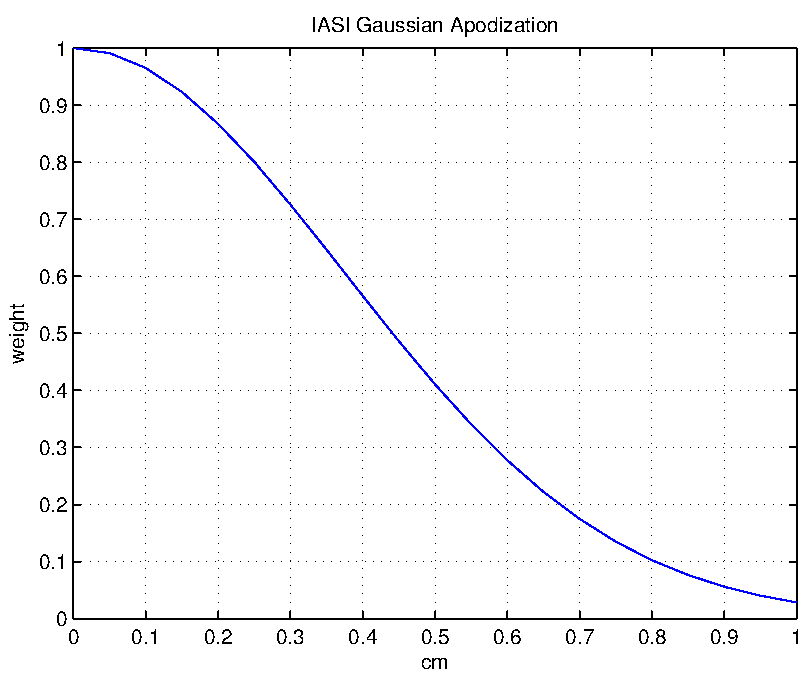
\includegraphics[height=8cm]{figures/iasi_gauss_app.pdf}
  \caption{{\iasi} truncated Gaussian apodization}
  \label{igauss}
\end{figure}

\begin{figure}
  \centering
  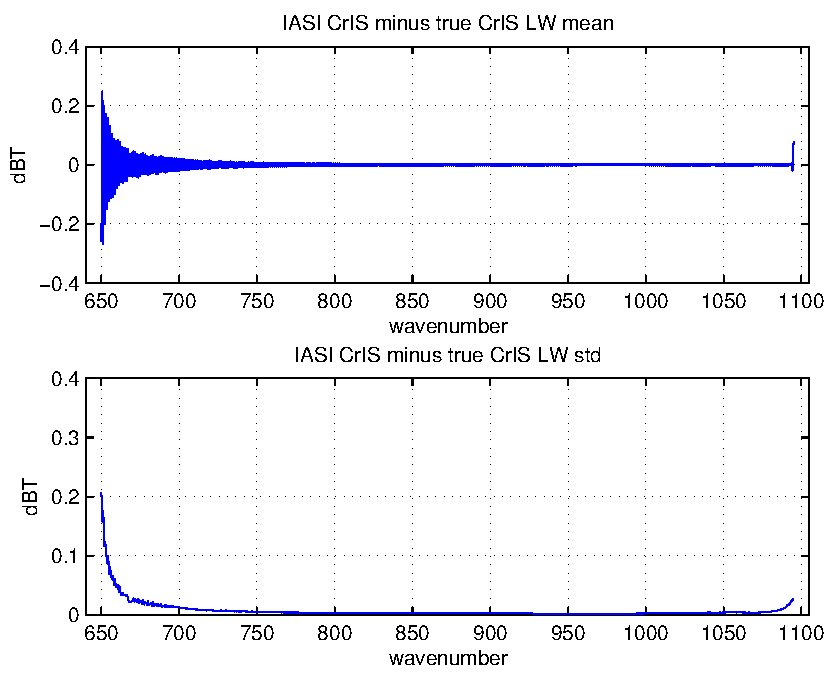
\includegraphics[height=8cm]{figures/iasi_cris_lw_1.pdf}
  \caption{Mean and standard deviation of unapodized {\iasi} {\cris}
    minus true {\cris}, for the {\cris} LW band.}
  \label{iclw1}
\end{figure}

\begin{figure}
  \centering
  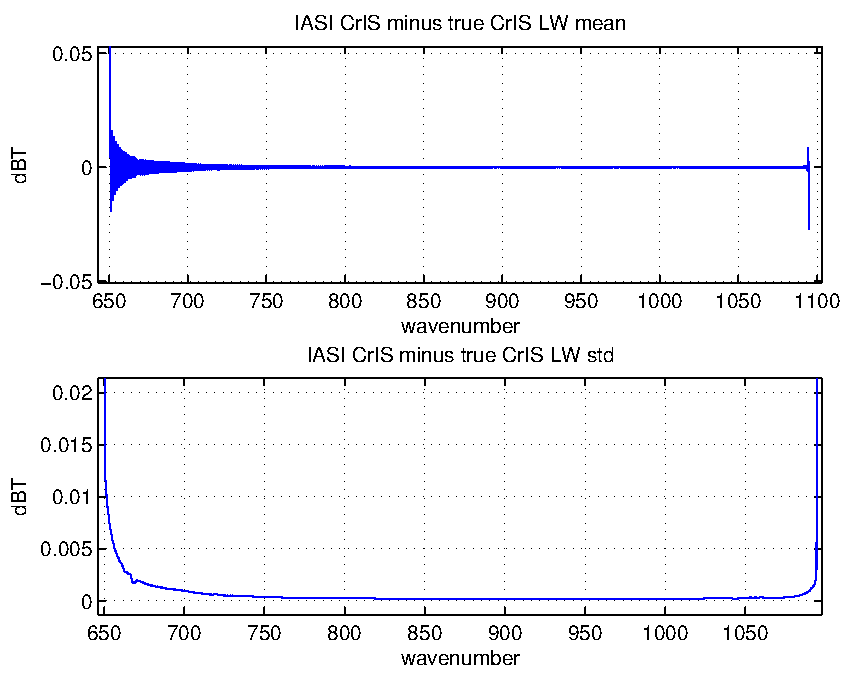
\includegraphics[height=8cm]{figures/iasi_cris_lw_2.pdf}
  \caption{Mean and standard deviation of Hamming apodized {\iasi}
    {\cris} minus true {\cris}, for the {\cris} LW band. }
  \label{iclw2}
\end{figure}

\begin{figure}
  \centering
  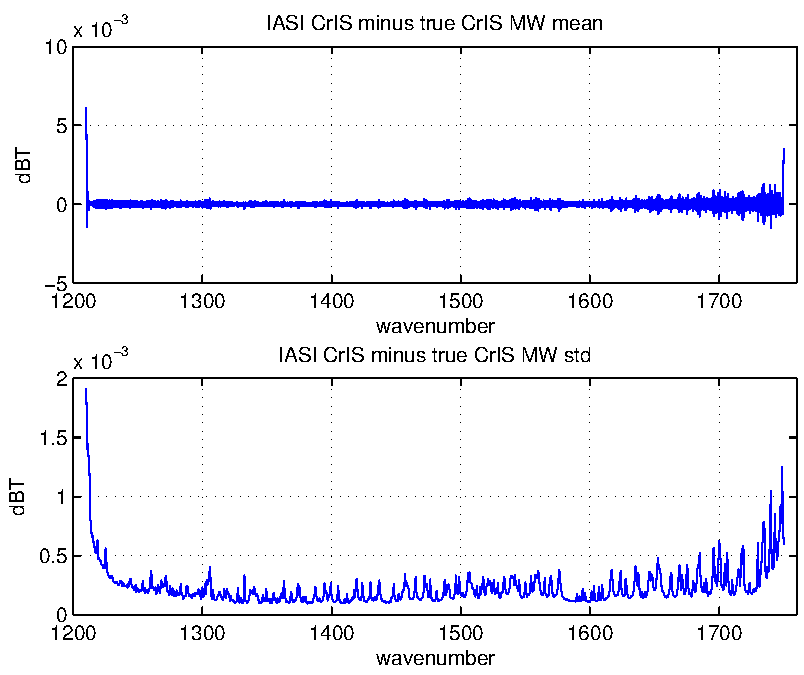
\includegraphics[height=8cm]{figures/iasi_cris_mw_1.pdf}
  \caption{Mean and standard deviation of unapodized {\iasi} {\cris}
    minus true {\cris}, for the {\cris} MW band.}
  \label{icmw1}
\end{figure}

\begin{figure}
  \centering
  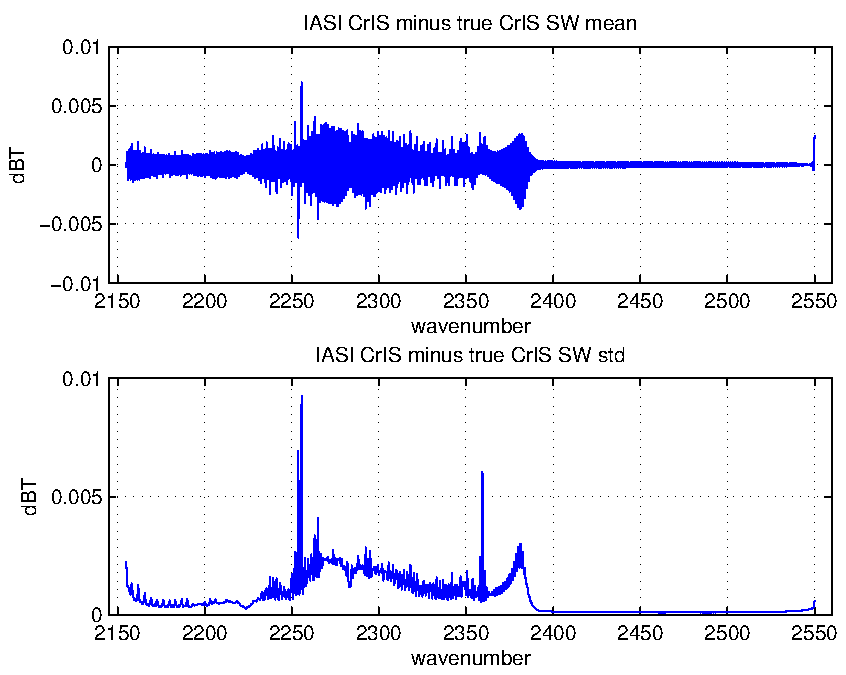
\includegraphics[height=8cm]{figures/iasi_cris_sw_1.pdf}
  \caption{Mean and standard deviation of unapodized {\iasi} {\cris}
    minus true {\cris}, for the {\cris} SW band.}
  \label{icsw1}
\end{figure}

\FloatBarrier


\section{IASI to AIRS}

{\airs} L1b radiances are a set of channels between approximately
650 to 2650 {\wn} with the individual center frequencies and
spectral response functions (SRFs) determined by the focal plane
geometery.  Channels are not uniformly spaced.  {\airs} L1c
radiances are derived from the L1b, with improvements including
filling the small gaps.  The {\iasi} to {\airs} translation will
work for either channel set, and is done as follows

% The {\iasi} to {\airs} translation applies a deconvolution to the
% full {\iasi} band, to a 0.1 {\wn} intermediate grid, and then an
% {\airs} convolution to get {\airs} channel radiances.  

\begin{itemize}

  \item apply a bandpass filter to the {\iasi} radiances to restrict
    them to the {\airs} band span, with a 5 {\wn} rolloff

  \item deconvolve the filtered {\iasi} radiances to a 0.1 {\wn}
    intermediate grid, the nominal resolution of the {\airs} SRF
    tabulation.  Aside from resolution and band spans, this exactly
    the same transform used for the {\iasi} to {\cris} translation

  \item convolve the 0.1 {\wn} intermediate representation with either
    the {\airs} L1b or L1c SRFs
    
\end{itemize}

Figure \ref{srfs1} shows the first three {\airs} SRFs and the
bandpass filter wing.  There is a tradeoff involved in the position
of the bandpass wing---the deconvolution is better behaved with a
broader wing, but we don't want to step on the wings of the AIRS
SRFs.

Figure \ref{iaspec} shows true {\iasi}, true {\airs}, 
deconvolved {\iasi}, and {\iasi} {\airs}.  At this level of detail
we mainly see the greater fine structure in the deconvolution.
Figure \ref{iadiff} shows {\iasi} {\airs} minus true {\airs}.  The
residual is larger than for the {\iasi} to {\cris} translation, but
significantly better than the {\airs} to {\cris} or {\cris} to
{\airs} translations.

\begin{figure}
  \centering
  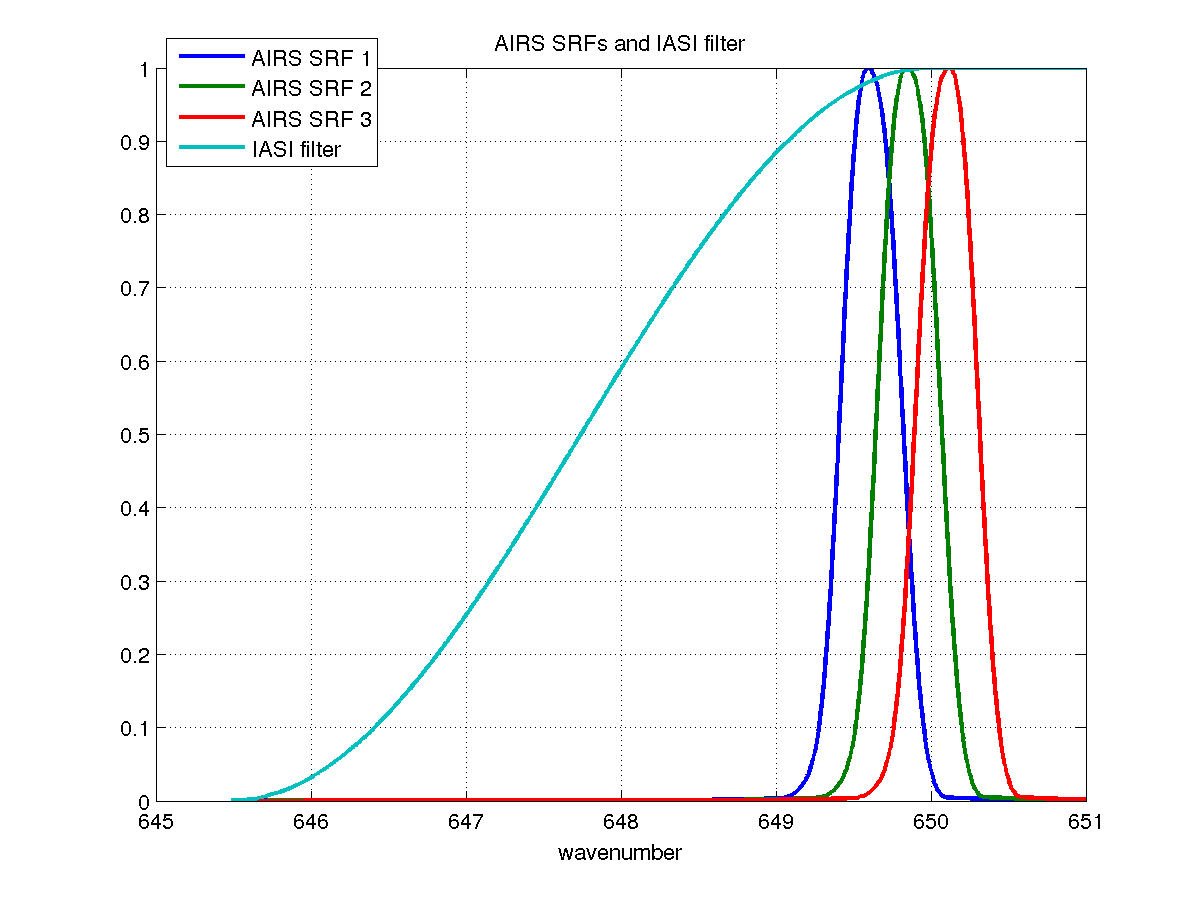
\includegraphics[height=8cm]{figures/srfs_and_filt.png}
  \caption{The first three {\airs} SRFs and the bandpass filter
    wing}
  \label{srfs1}
\end{figure}

\begin{figure}
  \centering
  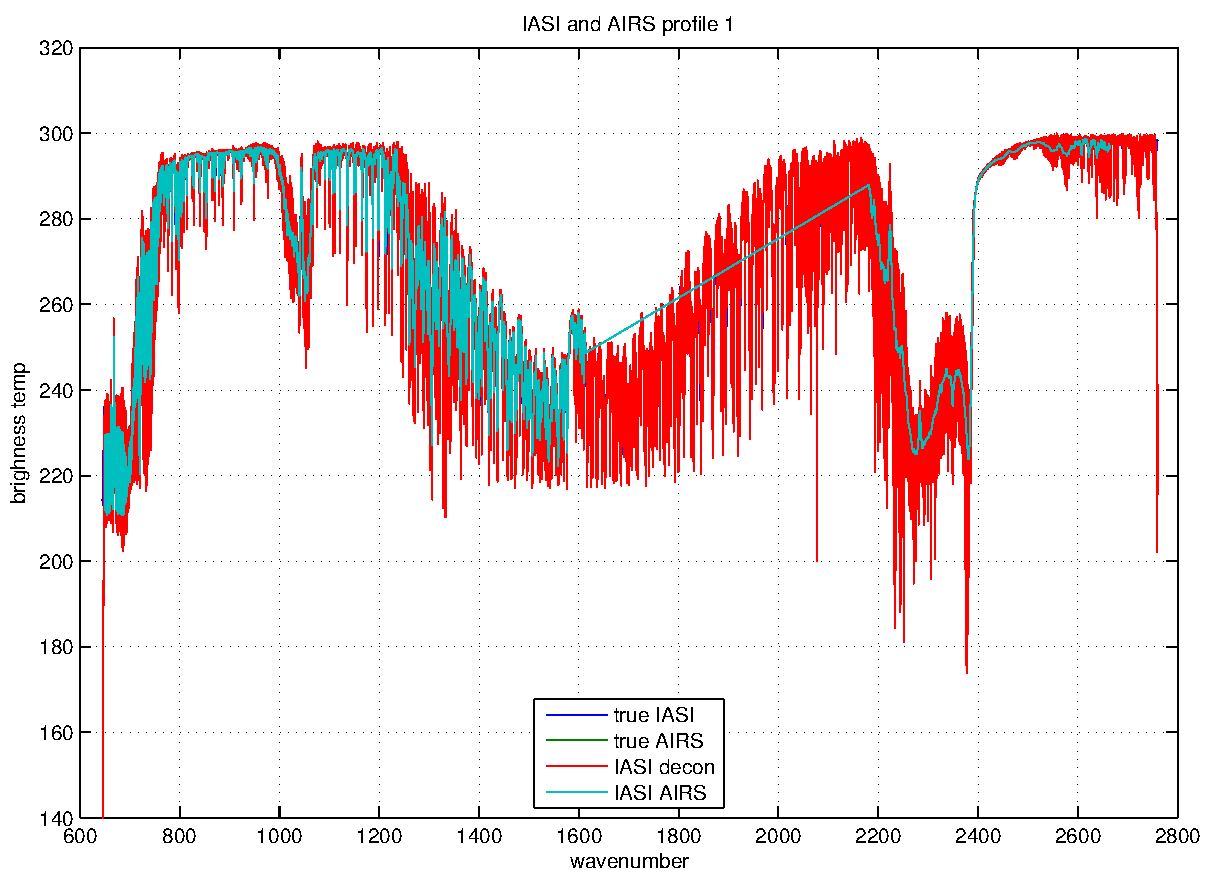
\includegraphics[height=8cm]{figures/iasi_airs_spec.pdf}
  \caption{true {\iasi}, true {\airs}, deconvolved {\iasi}, and
    {\iasi} {\airs} }
  \label{iaspec}
\end{figure}

\begin{figure}
  \centering
  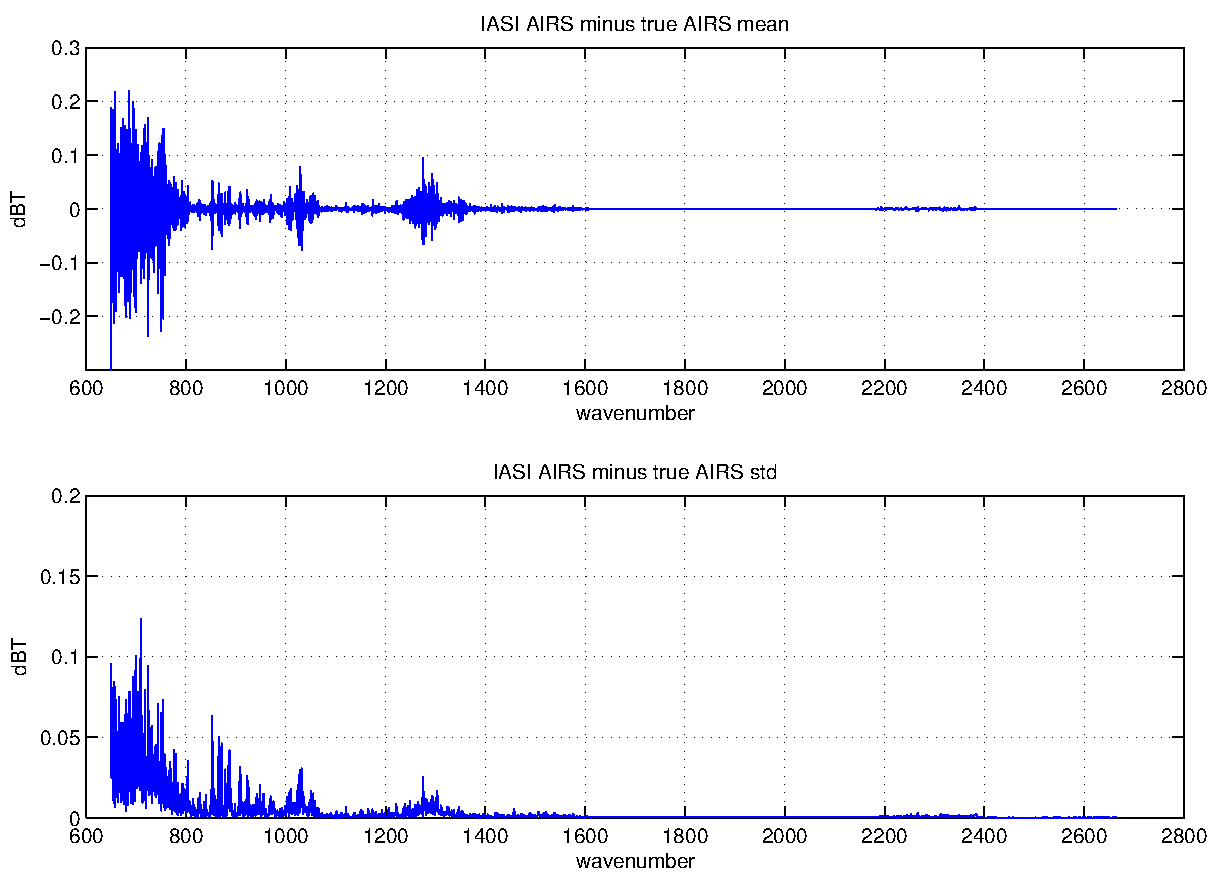
\includegraphics[height=8cm]{figures/iasi_airs_diff.pdf}
  \caption{Mean and standard deviation of {\iasi} {\airs} minus true
    {\airs} }
  \label{iadiff}
\end{figure}

\FloatBarrier

\section{AIRS to CrIS}

\section{CrIS to AIRS}

\end{document}
